\documentclass{article}

% Importing document settings from our file "packages.sty"
\usepackage{packages}

\fancyhead{} % clear all header fields
\fancyhead[LO]{\textbf{Vigdis-Irene Steinsund, \\ Thomas Hasvold}}
\fancyhead[CO]{\textbf{TDT4136 - Assignment 4}}
\fancyhead[RO]{\textbf{19/10/2023}}

% Beginning of document
\begin{document}

    % Defining main matter settings (Norsk: innstillinger for hoveddelen av teksten)
    \mainmatter

    \section*{Q2}

    \begin{figure}[H]
        \centering
        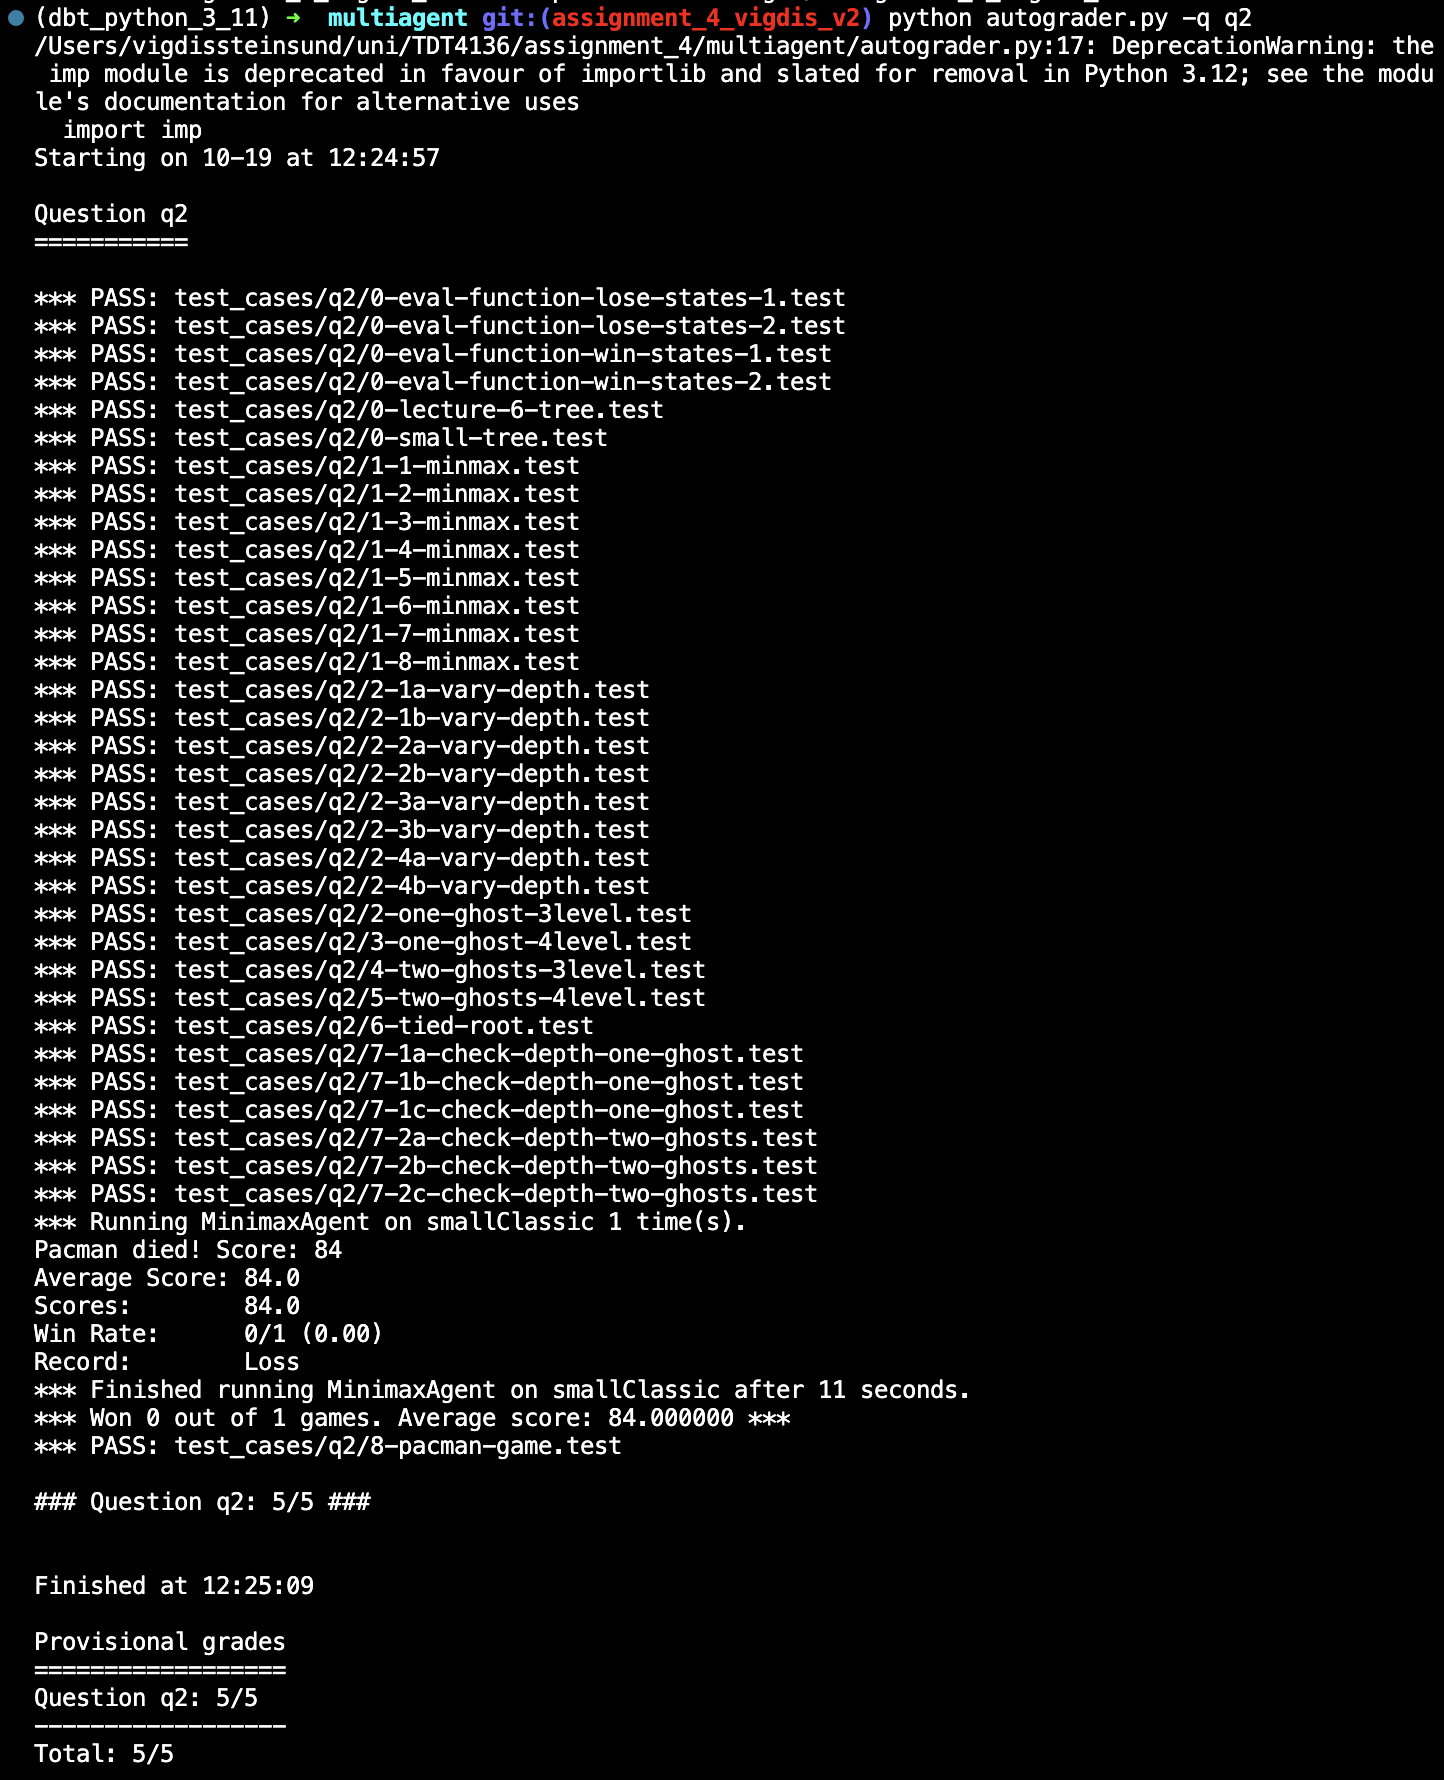
\includegraphics[width=0.8\textwidth]{Images/test_q2.png}
        \caption[Q2 test output]{Successful output from the autograder q2 task.}
        \label{fig:Q2 test output}
    \end{figure}

    \section*{Q3}

    \begin{figure}[H]
        \centering
        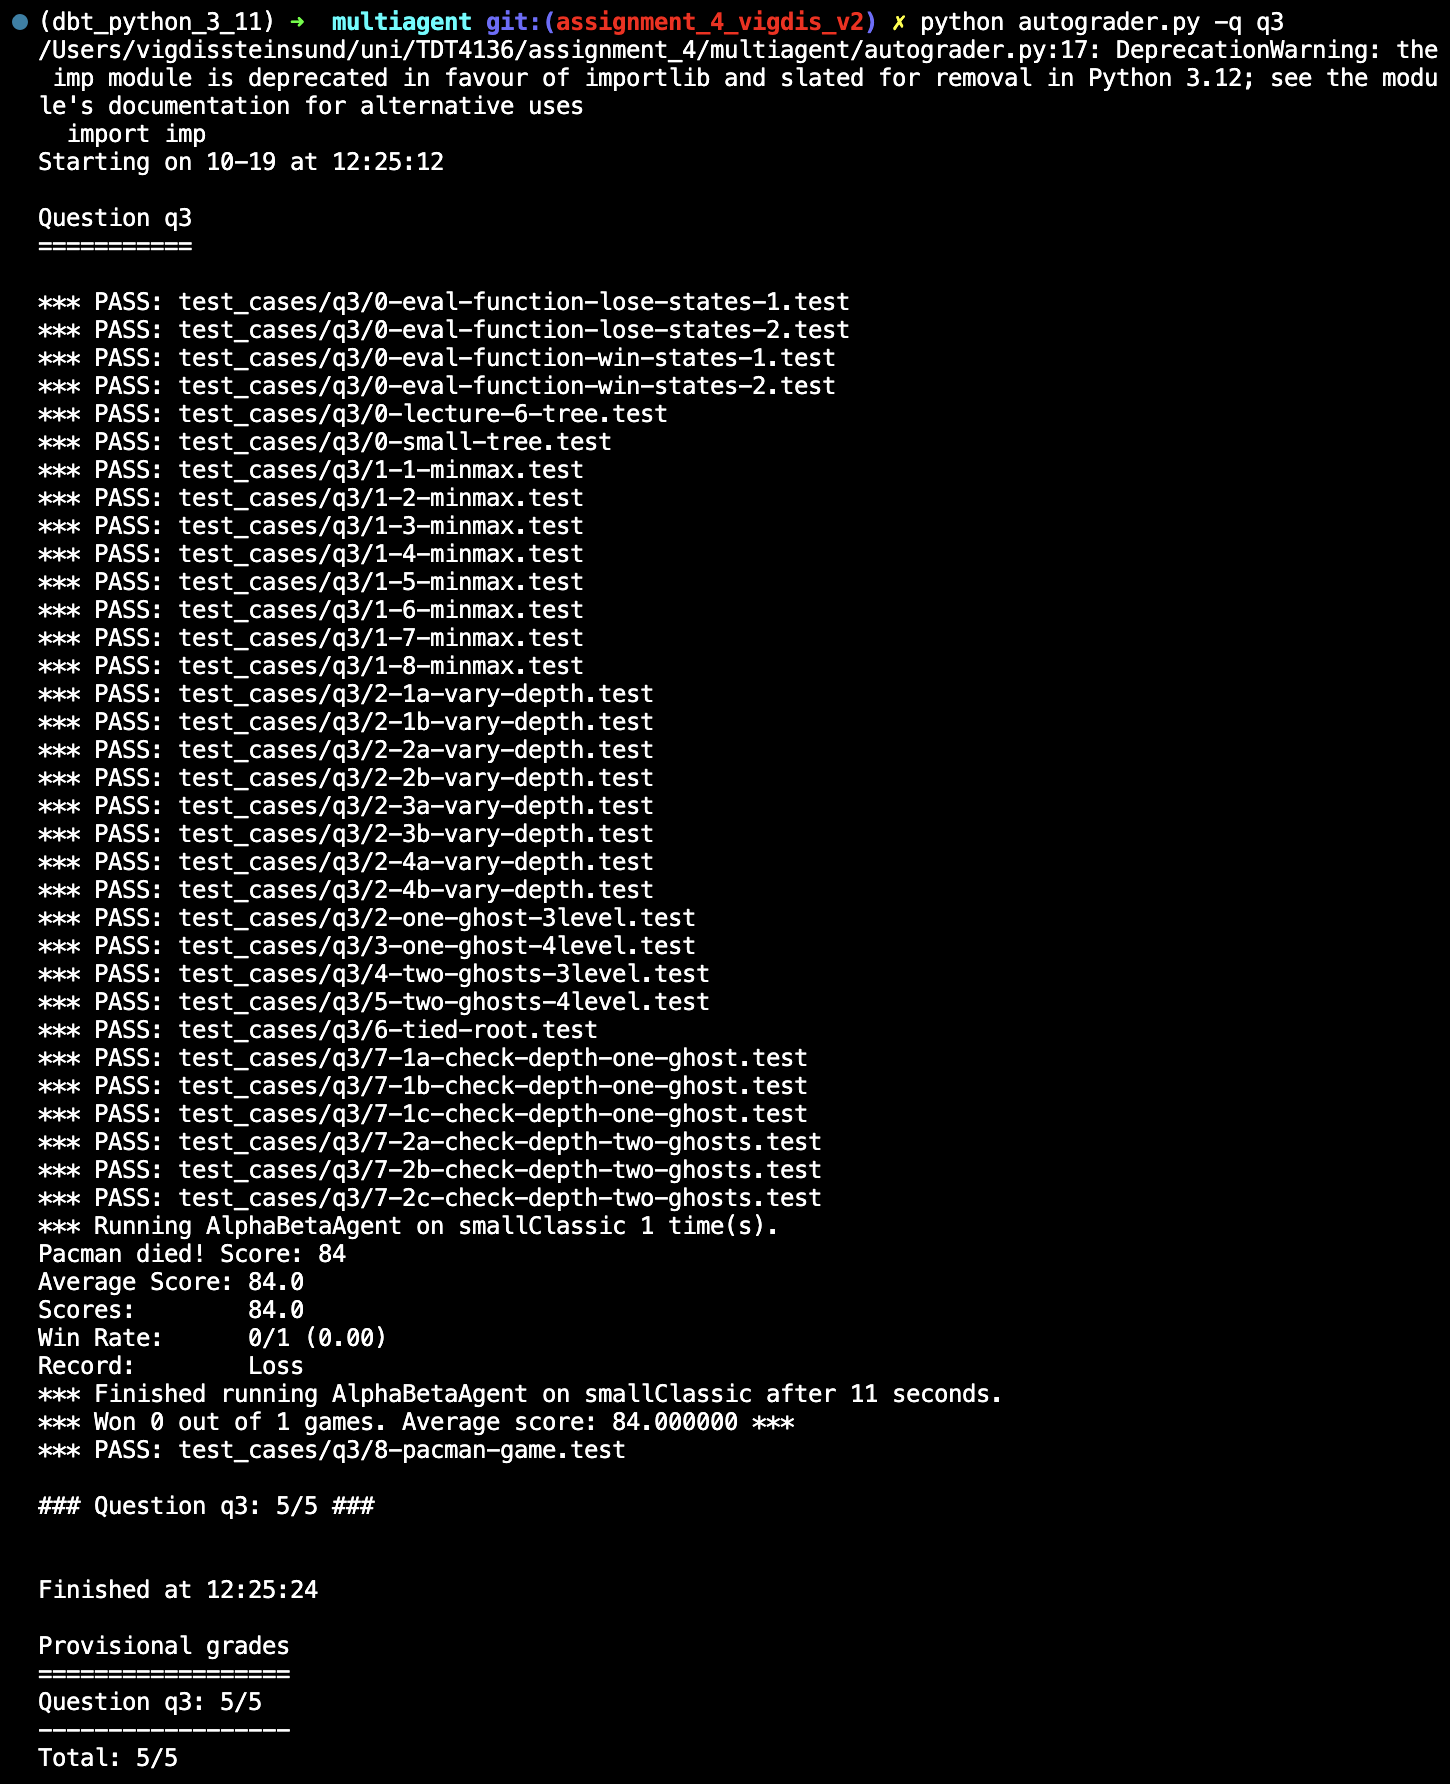
\includegraphics[width=0.8\textwidth]{Images/test_q3.png}
        \caption[Q3 test output]{Successful output from the autograder q3 task.}
        \label{fig:Q3 test output}
    \end{figure}

% End of document
\end{document}
